\documentclass[../main.tex]{subfiles}

\pagestyle{main}
\renewcommand{\chaptermark}[1]{\markboth{\chaptername\ \thechapter}{}}
\setcounter{chapter}{9}

\begin{document}




\chapter{Compactness}\label{sct:10}
\section{Journal}
\begin{definition}\label{dfn:10.1}\marginnote{2/23:}
    We say that a function $f:A\to\R$ is \textbf{bounded} if $f(A)$ is a bounded subset of $\R$. We say that $f$ is \textbf{bounded above} if $f(A)$ is bounded above and that $f$ is \textbf{bounded below} if $f(A)$ is bounded below.\par
    If $f:A\to\R$ is bounded above, we say that $f$ \textbf{attains} (its least upper bound) if there is some $a\in A$ such that $f(a)=\sup f(A)$. Similarly, if $f:A\to\R$ is bounded below, we say that $f$ \textbf{attains} (its greatest lower bound) if there is some $a\in A$ such that $f(a)=\inf f(A)$.
\end{definition}

\begin{exercise}\label{exr:10.2}
    If possible, find examples of each of the following: a picture suffices.
    \begin{enumerate}[label={\alph*)}]
        \item A continuous function on $[1,\infty)$ that is not bounded above.
        \begin{proof}[Example]
            Let $f:[1,\infty)\to\R$ be defined by $f(x)=x$.
            \begin{center}
                \begin{tikzpicture}
                    \footnotesize
                    \draw [->] (-0.4,0) -- (4,0) node[right]{$x$};
                    \draw [->] (0,-0.6) -- (0,3) node[above]{$y$};
                    \draw (1,0.1) -- ++(0,-0.2) node[below]{$1$};

                    \draw [thick,-stealth] (1,1) node[circle,fill,inner sep=1.5pt]{} -- (2.8,2.8);
                \end{tikzpicture}
            \end{center}
        \end{proof}
        \item A continuous function on $[1,\infty)$ that is bounded above but does not attain its least upper bound.
        \begin{proof}[Example]
            Let $f:[1,\infty)\to\R$ be defined by $f(x)=-\frac{1}{x}$.
            \begin{center}
                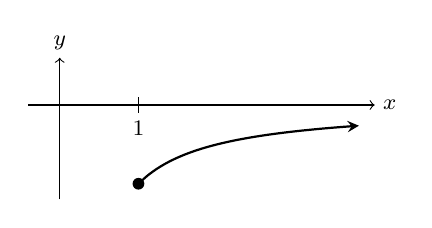
\begin{tikzpicture}
                    \footnotesize
                    \draw [->] (-0.4,0) -- (4,0) node[right]{$x$};
                    \draw [->] (0,-1.2) -- (0,0.6) node[above]{$y$};
                    \draw (1,0.1) -- ++(0,-0.2) node[below]{$1$};

                    \draw [thick,-stealth] plot [domain=1:3.8,smooth] (\x,{-1/\x});
                    \node [circle,fill,inner sep=1.5pt] at (1,-1) {};
                \end{tikzpicture}
            \end{center}
        \end{proof}
        \item A continuous function on $(0,1)$ that is not bounded below.
        \begin{proof}[Example]
            Let $f:(0,1)\to\R$ be defined by $f(x)=-\frac{1}{x}$.
            \begin{center}
                \begin{tikzpicture}
                    \footnotesize
                    \draw [->] (-0.4,0) -- (4,0) node[right]{$x$};
                    \draw [->] (0,-3) -- (0,0.6) node[above]{$y$};
                    \draw (1,0.1) -- ++(0,-0.2) node[below]{$1$};

                    \draw [thick,stealth-] plot [domain=0.36:1,smooth] (\x,{-1/\x}) node[circle,draw,thin,fill=white,inner sep=1.5pt]{};
                \end{tikzpicture}
            \end{center}
        \end{proof}
        \item A continuous function on $(0,1)$ that is bounded below but does not attain its greatest lower bound.
        \begin{proof}[Example]
            Let $f:(0,1)\to\R$ be defined by $f(x)=x$.
            \begin{center}
                \begin{tikzpicture}
                    \footnotesize
                    \draw [->] (-0.4,0) -- (4,0) node[right]{$x$};
                    \draw [->] (0,-0.6) -- (0,3) node[above]{$y$};
                    \draw (1,0.1) -- ++(0,-0.2) node[below]{$1$};

                    \draw [thick] (0,0) node[circle,draw,thin,fill=white,inner sep=1.5pt]{} -- (1,1) node[circle,draw,thin,fill=white,inner sep=1.5pt]{};
                \end{tikzpicture}
            \end{center}
        \end{proof}
    \end{enumerate}
\end{exercise}

\begin{definition}\label{dfn:10.3}
    Let $X$ be a subset of $\R$ and let $\mathcal{G}=\{G_\lambda\}_{\lambda\in\Lambda}$ be a collection of subsets of $\R$. We say that $\mathcal{G}$ is a \textbf{cover} of $X$ if every point of $X$ is in some $G_\lambda$, or in other words:
    \begin{equation*}
        X \subset \bigcup_{\lambda\in\Lambda}G_\lambda
    \end{equation*}
    We say that the collection $\mathcal{G}$ is an \textbf{open cover} if each $G_\lambda$ is open.
\end{definition}

\begin{definition}\label{dfn:10.4}
    Let $X$ be a subset of $\R$. $X$ is \textbf{compact} if for every open cover $\mathcal{G}$ of $X$, there exists a finite subset $\mathcal{G}'\subset\mathcal{G}$ that is also an open cover.
\end{definition}

A good summary of the definition of compactness is "every open cover contains a finite subcover."

\begin{exercise}\label{exr:10.5}
    Show that all finite subsets of $\R$ are compact.
    \begin{proof}
        Let $X$ be an arbitrary finite subset of $\R$. To prove that $X$ is compact, Definition \ref{dfn:10.4} tells us that it will suffice to show that for every open cover $\mathcal{G}$ of $X$, there exists a finite subset $\mathcal{G}'\subset\mathcal{G}$ that is also an open cover. Let $\mathcal{G}$ be an arbitrary open cover of $X$. By Definition \ref{dfn:10.3}, every point $x\in X$ is an element of $G_\lambda$ for some $G_\lambda\in\mathcal{G}$. Thus, for each $x\in X$, let $G_x\in\mathcal{G}$ be a set that contains $x$. Since $X$ is finite, we do not need the axiom of choice to make these selections. Additionally, since there are finitely many $X$, we know that there are finitely many distinct $G_x$\footnote{In fact, the number of $G_x$ is less than or equal to the cardinality of $X$ since we may choose the same $G_x$ for multiple $x$ but may not choose multiple $G_x$ for the same $x$.}. Thus, $\mathcal{G}'=\{G_x\}_{x\in X}$ is finite. Additionally, it is a subset of $\mathcal{G}$ by definition (each $G_x$ is defined to be an element of $\mathcal{G}$). Furthermore, each $G_x$ is open (again, each $G_x$ is an element of $\mathcal{G}$, which is a collection of open sets by definition). Lastly, every point $x\in X$ is an element of $G_x\in\mathcal{G}'$, so $\mathcal{G}'$ is a cover. Therefore, by Definition \ref{dfn:10.3}, $\mathcal{G}'\subset\mathcal{G}$ is a finite open cover of $X$.
    \end{proof}
\end{exercise}




\end{document}